\documentclass[fleqn,10pt]{wlscirep}
\usepackage{fixltx2e}
\usepackage{textcomp}
\usepackage{epstopdf}

\newcommand{\beginsupplement}{%
 \setcounter{table}{0}
 \renewcommand{\thetable}{S\arabic{table}}%
 \setcounter{figure}{0}
 \renewcommand{\thefigure}{S\arabic{figure}}%
 }

\title{Dendritic cells isolated from individuals susceptible to tuberculosis have an altered gene expression profile}


\author[1,2]{John D. Blischak}
\author[3]{Ludovic Tailleux}
\author[1]{Marsha Myrthil}
\author[4,5,*]{Luis B. Barreiro}
\author[1,6,*]{Yoav Gilad}



\affil[1]{Department of Human Genetics, University of Chicago, Chicago, Illinois, USA}
\affil[2]{Committee on Genetics, Genomics, and Systems Biology, University of Chicago, Chicago, Illinois, USA}
\affil[3]{Mycobacterial Genetics Unit, Institut Pasteur, Paris, France}
\affil[4]{Department of Genetics, CHU Sainte-Justine Research Center, Montreal, Québec, Canada}
\affil[5]{Department of Pediatrics, University of Montreal, Montreal, Québec, Canada}
\affil[6]{Department of Medicine, University of Chicago, Chicago, Illinois, USA}



\affil[*]{Correspondence should be addressed to YG (gilad@uchicago.edu) and LBB (luis.barreiro@umontreal.ca).}

\begin{abstract}
Write abstract here…
\end{abstract}
\begin{document}
\flushbottom
\maketitle
\thispagestyle{empty}

\section*{Introduction}

\section*{Results}

\subsection*{Susceptible individuals have an altered transcriptome in the noninfected state}

We obtained whole blood samples from 25 healthy individuals. Six of
the donors had recovered from a previous active TB infection, and are
thus susceptible. The remaining 19 tested positive for a latent TB
infection without ever experiencing symptoms of active TB, and are
thus resistant. We isolated dendritic cells (DCs) and treated them
with \emph{Mycobacterium }\emph{tuberculosis} (MTB) or a mock control.
To measure genome-wide gene expression levels, we sequenced the RNA at
18 hours post-infection, using a processing pipeline designed to
minimize the introduction of unwanted technical variation, and
obtained a mean of X $\pm$ X million raw reads per sample. We
performed quality control analyses to remove non-expressed genes
(Supplementary Fig. \ref{fig:gene}), identify and remove outliers
(Supplementary Fig. \ref{fig:outliers}), and check for confounding
batch effects (Supplementary Fig. \ref{fig:batch},
\ref{fig:infection}). Ultimately 6 samples were removed from all
downstream analyses (Supplementary Fig. \ref{fig:outliers}).

Next we performed a standard differential expression analysis using a
linear modeling framework, defined in equation (\ref{eq:limma}). As
expected, there was a strong response to infection with MTB in both
resistant and susceptible individuals (Supplementary Fig.
\ref{fig:limma-supp}). 3,486 genes were differentially expressed (DE)
between the noninfected and infected states for resistant individuals
at a q-value of 10\% and an absolute log fold change greater than 1.
Similarly, 3,789 genes were DE between the noninfected and infected
states for resistant individuals at a q-value of 10\% and an absolute
log fold change greater than 1. These genes included the important
immune response factors \emph{IL12B}, \emph{REL}, and \emph{TNF}. Of
most interest were genes which were DE between susceptible and
resistant individuals in the noninfected or infected states (Fig.
\ref{fig:limma}). 645 genes were DE between resistant and susceptible
individuals in the noninfected state at a q-value of 10\%, including
\emph{ATPV1B2}, \emph{FEZ2}, \emph{PSMA2}, \emph{TNFRSF25}, and
\emph{TRIM38}. 0 genes were DE between resistant and susceptible
individuals in the noninfected state at a q-value of 10\%.

\begin{figure}[p]
\centering
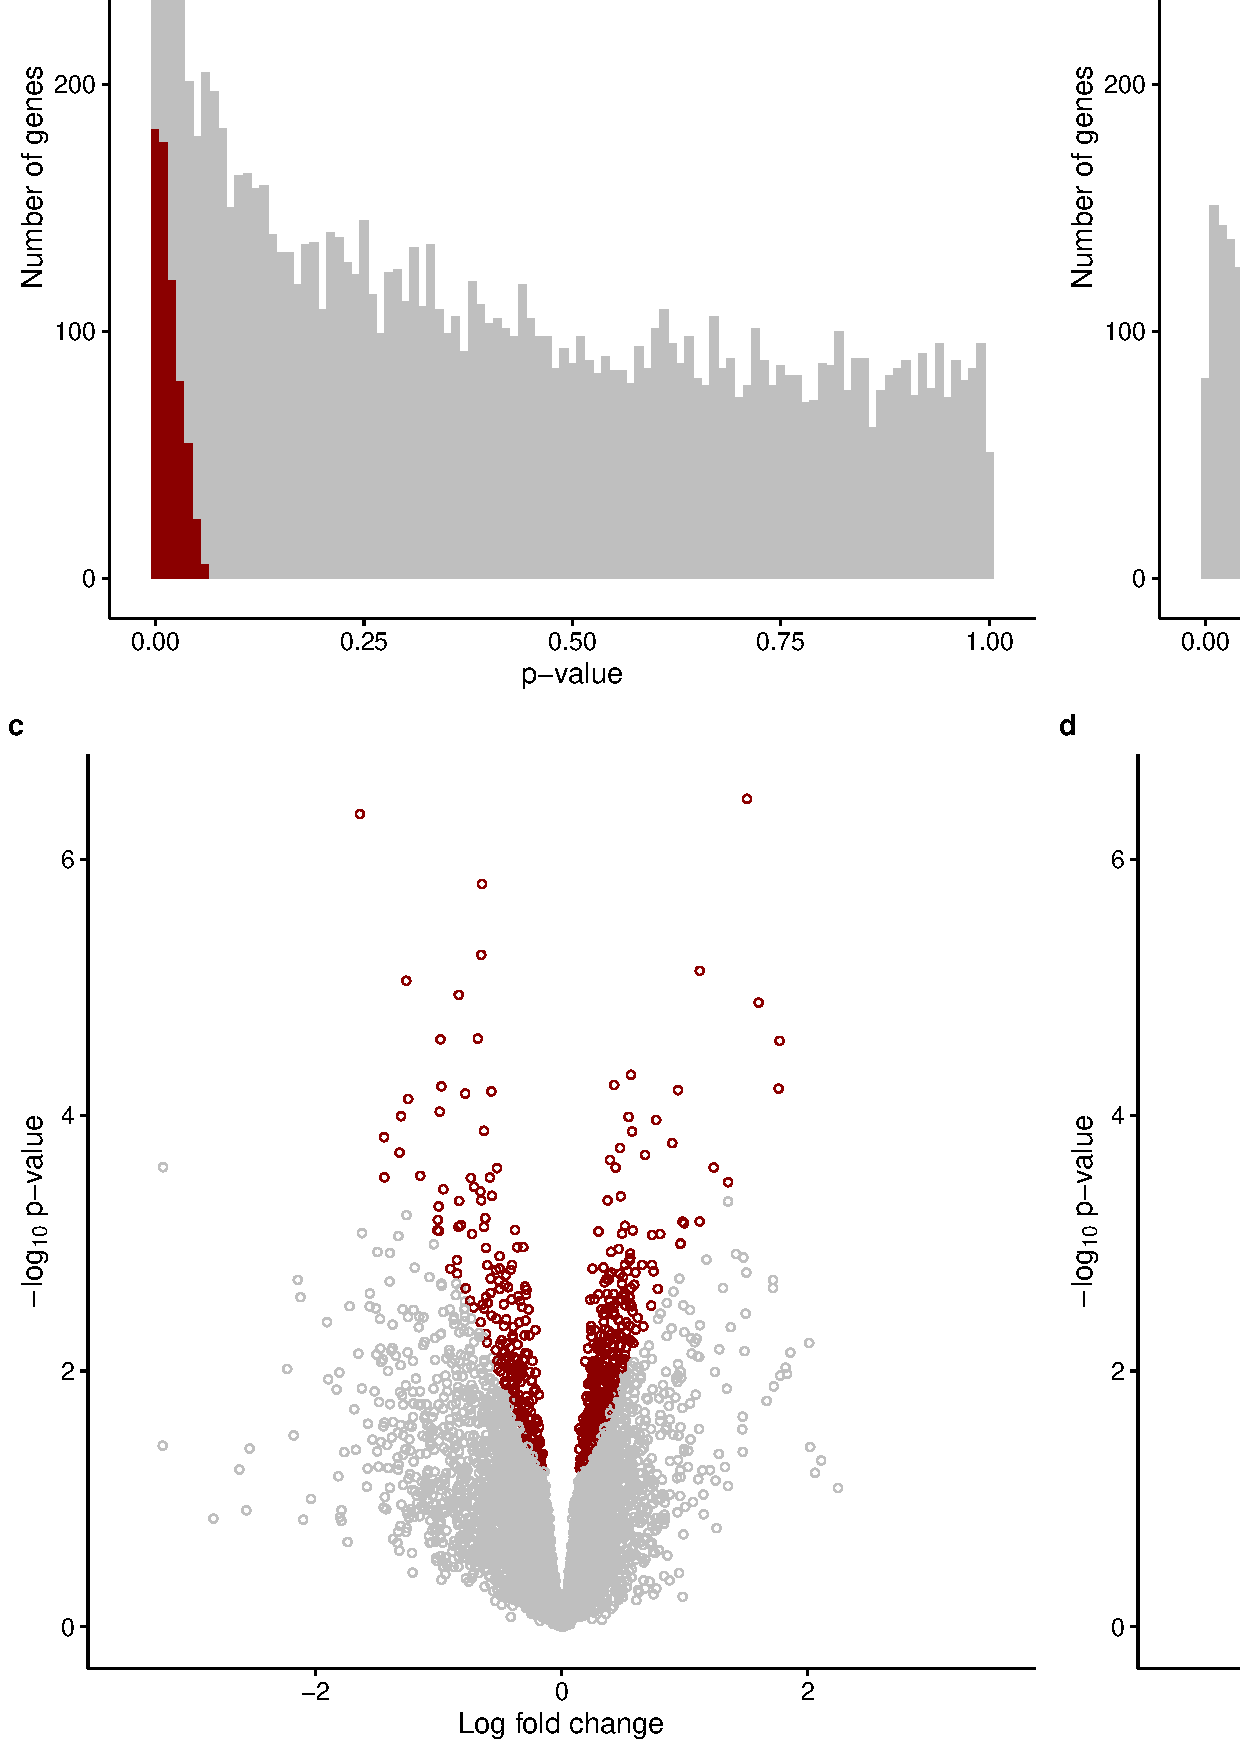
\includegraphics[width=\linewidth]{../figure/limma.pdf}
\caption{
Differential expression analysis. The top panel contains the
distribution of unadjusted p-values after testing for differential
expression between susceptible and resistant individuals in the (a)
noninfected or (b) infected state. The bottom panel contains the
corresponding volcano plots for the (c) noninfected and (d) infected
states. The x-axis is the log fold change in gene expression level
between susceptible and resistant individuals and the y-axis is the
–log\textsubscript{10} p-value. Red indicates genes which are
significant differentially expressed with a q-value less than 10\%.
}
\label{fig:limma}
\end{figure}
\subsection*{Differentially expressed genes are enriched for TB susceptibility loci}

We next sought to investigate whether the differentially expressed
genes we had identified in our \emph{in vitro} experimental system
were important for the genetic basis of TB susceptibility. To do this,
we compared our results to TB susceptibility GWAS conducted in The
Gambia and Ghana \cite{Thye2010}. Specifically, for each gene we
assigned the SNP with the lowest p-value among all SNPs located within
50 kb of its transcription start site (TSS). If the differentially
expressed genes are enriched for TB susceptibility loci, we expect a
negative correlation between the absolute values of the log fold
changes in our experiment and the GWAS p-values. Indeed, this is what
we observed (Fig. \ref{fig:gwas}). We fit a line using least squares
regression for each of our differential expression tests.
Interestingly, we observed the steepest negative slopes for the tests
comparing differential expression between susceptible and resistant
individuals in the noninfected or infected states (Fig.
\ref{fig:gwas}b). However, the slopes of the best fit lines for the
tests of the effect of treatment in either resistant or susceptible
individuals were also negative. Of particular interest as potential
genes involved in TB susceptibility are the genes with that had a
p-value less than 0.01 in both The Gambia and Ghana GWAS and an
absolute log fold change greater than 2 between susceptible and
resistant individuals in the noninfected state (Fig. \ref{fig:gwas}a).
Only 2 genes met these criteria: \emph{CCL1} and \emph{UNC13A}.

\begin{figure}[ht]
\centering
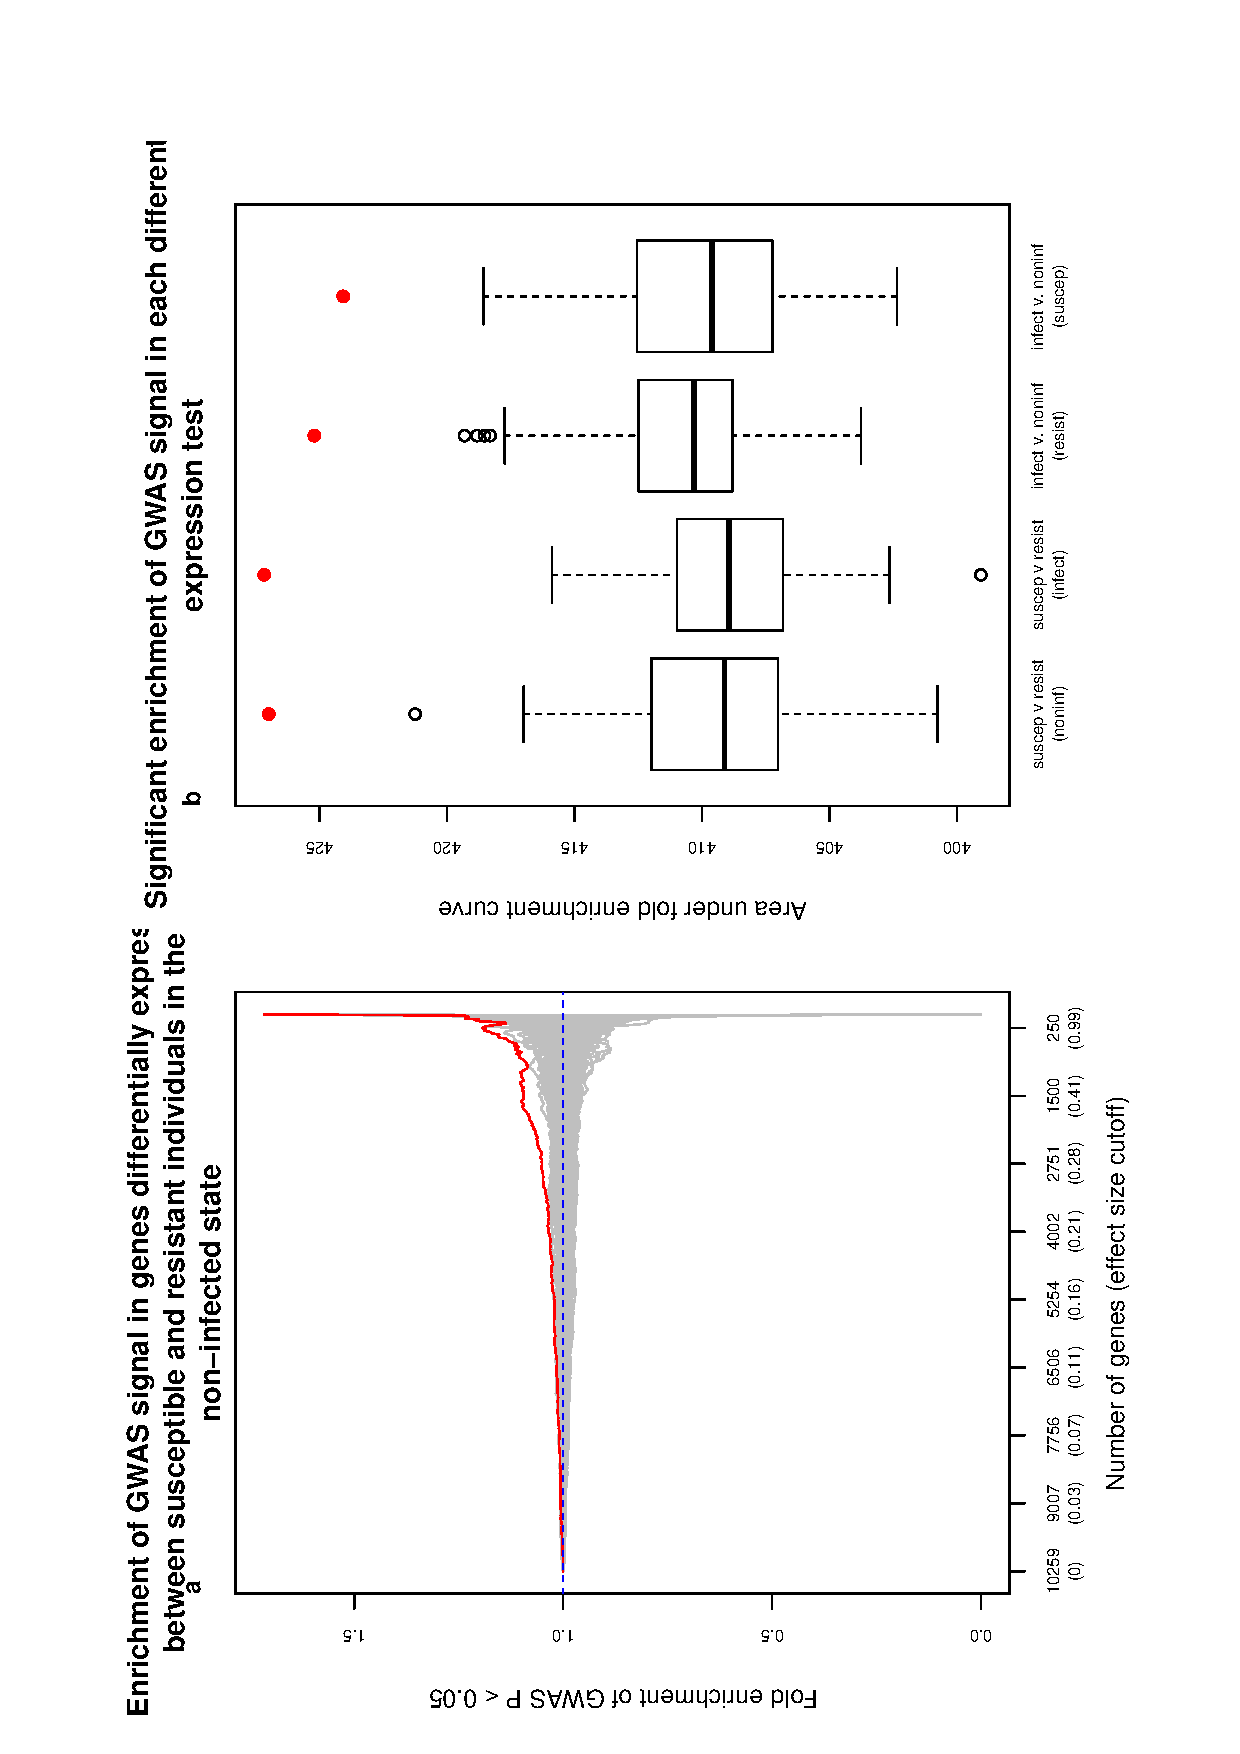
\includegraphics[width=\linewidth]{../figure/gwas.pdf}
\caption{
Comparison of differential expression and GWAS results. (a) The
relationship between p-values from the GWAS in The Gambia
\cite{Thye2010} and the absolute values of the log fold changes
between susceptible and resistant individuals in the noninfected
state. The red line is the least squares regression. (b) The slopes
($\pm$ 2x standard error) of the regression lines for each test. The
results from the GWAS in Gambia are in red and those from Ghana in
blue. All slopes are significantly different than 0 (t-test \emph{P}
\textless \, 0.05), except for the slope between the Ghana GWAS
p-values and the absolute values of the log fold changes between
susceptible and resistant individuals in the noninfected state.
}
\label{fig:gwas}
\end{figure}

\subsection*{Gene expression levels in the noninfected state can predict susceptibility status}

Next we attempted to build a gene expression based classifier to
predict susceptibility status. We focused on the gene expression
levels measured in the noninfected state both because this is where we
observed the largest differences between susceptible and resistant
individuals (Fig. \ref{fig:limma}ac) and also since it is much more
practical to obtain gene expression data from noninfected DCs compared
to MTB-infected DCs. We trained a support vector machine using the 99
genes that were differentially expressed between resistant and
susceptible individuals in the noninfected state at a q-value less
than 5\% (see Methods for a full description of how we selected this
model). Encouragingly, we observed a clear separation between
susceptible and resistant individuals when comparing the predicted
probability of being resistant to TB for each sample obtained from
leave-one-out-cross-validation (Fig. \ref{fig:classifier}a). Using a
cutoff of 0.75 for the predicted probability of being resistant to TB,
we obtained a sensitivity of 100\% (5 out of 5 susceptible individuals
classified as susceptible) and a specificity of \texttildelow71\% (5
out of 7 individuals classified as susceptible were true positives).

Unfortunately our current data set was too small to properly split
into separate training and testing sets. In order to assess the
plausibility of our model, we applied the classifier to an independent
study which collected genome-wide gene expression levels in DCs from
65 healthy individuals \cite{Barreiro2012}. Using the same cutoff of
0.75 for the probability of being resistant to TB that was determined
to be optimal in the training set, \texttildelow11\% (7 out of 65) of
the individuals were classified as being susceptible to TB, similar to
the general estimate that 10\% of the population is susceptible to TB
(Fig. \ref{fig:classifier}b).

\begin{figure}[ht]
\centering
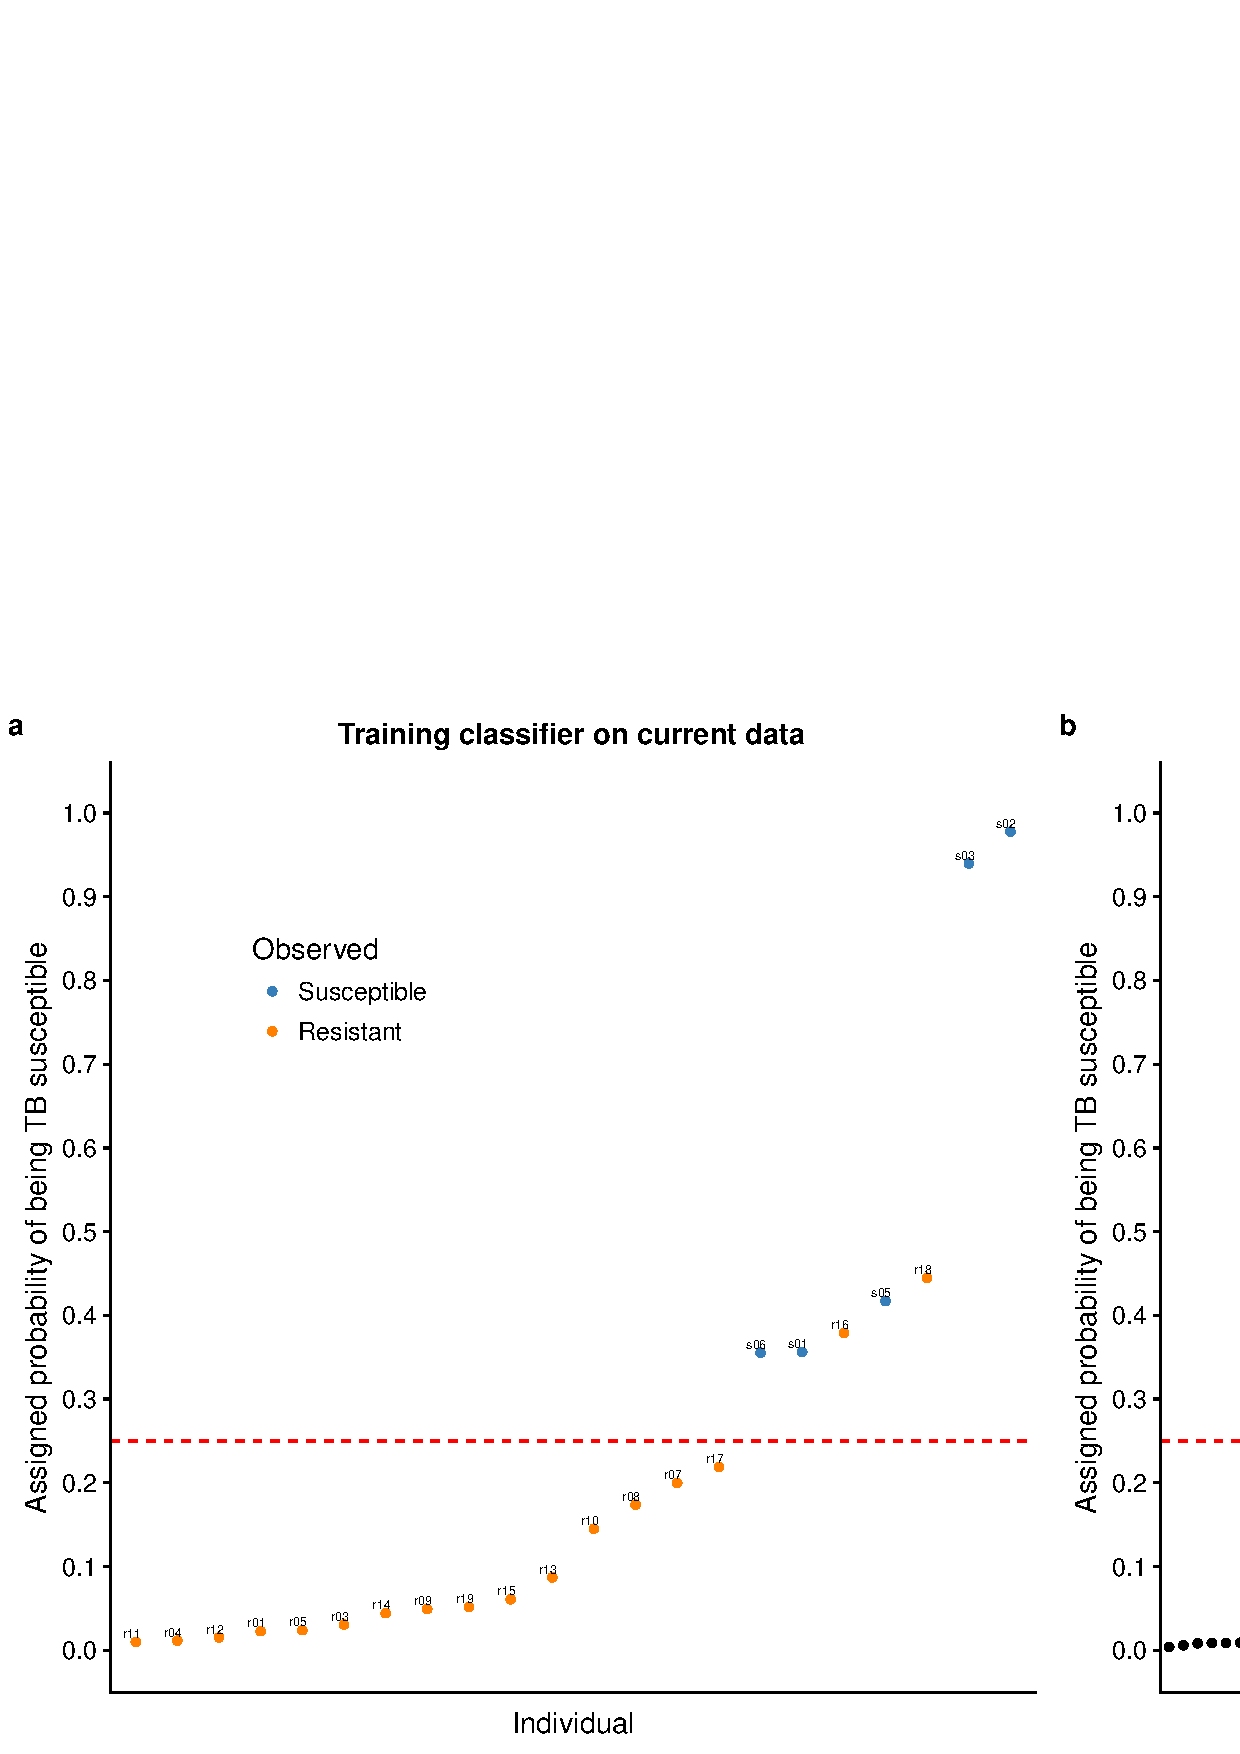
\includegraphics[width=\linewidth]{../figure/classifier-svm.pdf}
\caption{
Classifying TB susceptible individuals using a support vector machine
model. (a) The estimates of predicted probability of TB resistance
from the leave-one-out-cross-validation for individuals in the current
study. The red circles represent individuals known to be susceptible
to TB, and blue those resistant to TB. The horizontal dashed red line
at a probability of 0.75 separates susceptible and resistant
individuals. (b) The estimates of predicted probability of TB
resistance from applying the classifier trained on the data from the
current study to a test set of independently collected healthy
individuals \cite{Barreiro2012}.
}
\label{fig:classifier}
\end{figure}

\section*{Discussion}

Some ideas below…but not finished yet.

We obtained dendritic cells (DCs) from individuals that were known to
be susceptible or resistant to developing active tuberculosis (TB) and
measured genome-wide gene expression levels 18 hours post-infection
with \emph{Mycobacterium tuberculosis} (MTB) and noninfected controls.
Interestingly, we identified X genes which were differentially
expressed between susceptible and resistant individuals in the
noninfected state, including X, Y, and Z (Fig. \ref{fig:limma}.
Furthermore, we found that these differentially expressed genes were
enriched for low GWAS p-values (Fig. \ref{fig:gwas}) and could be used
to classify susceptible and resistant individuals.

Previous work in TB \cite{Thuong2008}
Previous work using gene expression to understand susceptibility
\cite{Bryant2014}

Overall our promising results in this small study suggest that
collecting blood samples from a larger cohort of susceptible
individuals would enable building a gene expression based classifier
able to confidently assess risk of TB susceptibility. By reducing the
number of resistant individuals receiving treatment for a latent TB
infection, we can eliminate the adverse health effects of a 6 month
regimen of antibiotics for these individuals and also reduce the
selective pressures on MTB to develop drug resistance.
\section*{Methods}

\subsection*{Ethics Statement}

We recruited 25 subjects to donate a blood sample for use in our
study. All methods were carried out in accordance with relevant
guidelines and regulations. The experimental protocols were approved
by the Institutional Review Boards of the University of Chicago
(10-504-B) and the Institut Pasteur (IRB00006966). All study
participants provided written informed consent.
\subsection*{Sample collection}

We collected whole blood samples from healthy Caucasian male
individuals living in France. The putatively resistant individuals
tested positive for a latent TB infection in an interferon-$\gamma$
release assay, but had never developed active TB. The putatively
sensitive individuals had developed active TB in the past, but were
currently healthy.
\subsection*{Isolation and infection of dendritic cells}

We isolated mononuclear cells from the whole blood samples using
Ficoll-Paque centrifugation, extracted monocytes via CD14 positive
selection, and differentiated the monocytes into dendritic cells (DCs)
by culturing them for 5 days in RPMI 1640 (Invitrogen) supplemented
with 10\% heat-inactivated FCS (Dutscher), L-glutamine (Invitrogen),
GM-CSF (20 ng/mL; Immunotools), and IL-4 (20 ng/mL; Immunotools). Next
we infected the DCs with \emph{Mycobacterium tuberculosis} (MTB) H37Rv
at a multiplicity of infection of 1-to-1 for 18 hours.
\subsection*{RNA extraction and sequencing}

We extracted RNA using the Qiagen miRNeasy Kit and prepared sequencing
libraries using the Illumina TruSeq Kit. We sent the master mixes to
the University of Chicago Functional Genomics Facility to be sequenced
on an Illumina HiSeq 4000. We designed the batches for RNA extraction,
library preparation, and sequencing to balance the experimental
factors of interest and thus avoid potential technical confounders
(Supplementary Fig. \ref{fig:process}).
\subsection*{Read mapping}

We mapped reads to human genome hg38 (GRCh38) using Subread and
discarded non-uniquely mapping reads. We downloaded the exon
coordinates of 19,800 Ensembl protein-coding genes (Ensembl 83, Dec
2015, GRCh38.p5) using the R/Bioconductor package biomaRt and assigned
mapped reads to these genes using featureCounts.
\subsection*{Quality control}

First we filtered genes by their expression level by removing all
genes with a median log\textsubscript{2} counts per million (cpm) less
than zero. This resulted in a final set of 11,336 genes for downstream
analysis (Supplementary Fig. \ref{fig:gene}, Supplementary Data S1).
Next we used principal components analysis (PCA) and hierarchical
clustering to identify and remove 6 outliers (Supplementary Fig.
\ref{fig:heat-all}, \ref{fig:heat-filt}, \ref{fig:outliers}). We did
this systematically by removing any sample that did not fall within
the mean $\pm$ two standard deviations of the first six PCs.
Furthermore, for the first PC which separated the samples by
treatment, we calculated a separate mean for the noninfected and
infected samples.

After filtering lowly expressed genes and removing outliers, we
recalculated the PCA to check for any potential confounding technical
batch effects (Supplementary Fig. \ref{fig:batch}). Reassuringly, the
major sources of variation in the data were from the biological
factors of interest. PC1 was strongly correlated with the effect of
treatment, and PCs 2-6 were correlated with inter-individual
variation. The only concerning technical factor was the infection
experiments, which were done in 12 separate batches (Supplementary
Fig. \ref{fig:process}). Infection batch correlated with PCs 3 and 5;
however, we verified that this variation was not confounded with our
primary outcome of interest, TB susceptibility (Supplementary Fig.
\ref{fig:infection}).
\subsection*{Differential expression analysis}

We used limma+voom \cite{Smyth2004, Law2014, Ritchie2015} to implement
the following linear model to test for differential expression:
\begin{equation} \label{eq:limma}
Y\ \sim \beta_{0} + X_{treat}\beta_{treat} + X_{status}\beta_{status} + X_{treat,status}\beta_{treat,status} + I + \epsilon
\end{equation}
where $\beta_{0}$ is the mean expression level in noninfected cells of
resistant individuals, $\beta_{treat}$ is the fixed effect of
treatment in resistant individuals, $\beta_{status}$ is the fixed
effect of susceptibility status in noninfected cells,
$\beta_{treat,status}$ is the fixed interaction effect of treatment in
susceptible individuals, and $I$ is the random effect of individual.
The random individual effect was implemented using the limma function
duplicateCorrelation (cite paper). To jointly model the data with voom
and duplicateCorrelation, we followed the recommended best practice of
running both voom and duplicateCorrelation twice in succession (cite
Lui2015).

We used the model to test 4 separate hypotheses (Supplementary Data
S2). We identified genes which were differentially expressed between
infected and noninfected DCs of resistant individuals by testing
$\beta_{treat} = 0$, genes which were differentially expressed between
infected and noninfected DCs of susceptible individuals by testing
$\beta_{treat} + \beta_{treat,status} = 0$, genes which were
differentially expressed between susceptible and resistant individuals
in the noninfected state by testing $\beta_{status} = 0$, and genes
which were differentially expressed between susceptible and resistant
individuals in the infected state by testing $\beta_{status} +
\beta_{treat,status} = 0$. We corrected for multiple testing using
q-values estimated via adaptive shrinkage \cite{Stephens2016} and
considered differentially expressed genes as those with a q-value less
than 10\%.
\subsection*{Comparison to GWAS results}

The GWAS p-values were from a study of TB susceptibility conducted in
The Gambia and Ghana \cite{Thye2010}. To compare our differential
expression results to these genetic associations, we assigned each
gene the p-value of the SNP with the minimum p-value out of all the
SNPs located within 50 kb up or downstream of its transcription start
site. Specifically, we obtained the genomic coordinates of the SNPs
with the R/Bioconductor package SNPlocs.Hsapiens.dbSNP144.GRCh38 and
matched SNPs to nearby genes using GenomicRanges. 10,260 of the 11,336
were assigned an association p-value. For each of the 4 hypotheses we
tested, we performed least squares regression of the differential
expression effect sizes (the log fold changes) and the assigned GWAS
p-values. We assessed the statistical significance of these
regressions using the standard t-test and reported the slope of each
regression line (Fig. \ref{fig:gwas}, Supplementary Data S3).  Lastly,
we also observed a negative correlation between the GWAS p-value
assigned to a gene and the number of SNPs tested nearby that gene
(Supplementary Fig. \ref{fig:gwas-n-snps}). However, we could not
think of an explanation for why genes with a larger log fold change in
our \emph{in vitro} experimental system would have more nearby genetic
variation, and thus we do not believe this relationship biased our
observation of a negative correlation between GWAS p-value and log
fold change.
\subsection*{Classifier}

The training set included the 44 high-quality noninfected samples from
this study with known susceptibility status. The test set included the
65 noninfected samples from one of our previous studies in which the
susceptibility status is unknown \cite{Barreiro2012}, and thus assumed
to be similar to that in the general population (\texttildelow10\%).
Because the two studies are substantially different, we took multiple
steps to make them comparable. First, we subset to include only those
9,450 genes which were assayed in both. Second, because the dynamic
range obtained from RNA-seq (current study) and microarrays (previous
study \cite{Barreiro2012}) were very different, we normalized the gene
expression levels to a standard normal with $\mu = 0$ and $\sigma = 1$
(Supplementary Fig. \ref{fig:combined-dist}). Third, we corrected for
the large, expected batch effect between the two studies by regressing
out the first principal component (PC) of the combined expression data
using the limma function removeBatchEffect \cite{Ritchie2015}
(Supplementary Fig. \ref{fig:combined-pca}).

To identify genes to use in the classifier, we performed a
differential expression analysis on the normalized, batch-corrected
data from the current study using the same approach described above
(with the exception that we no longer used voom since the data were no
longer counts). Specifically, we tested for differential expression
between susceptible and resistant individuals in the noninfected state
and identified sets of genes to use in the classifer by varying the
q-value cutoff. Cutoffs of 5\%, 10\%, 15\%, 20\%, and 25\%
corresponded to gene set sizes of 99, 385, 947, 1,934, and 3,697,
respectively. We used the R package caret (cite) to train 3 different
machine learning models: elastic net (cite glmnet), support vector
machine, and random forest (the parameters for each individual model
were selected using the Kappa statistic). To assess the results of the
model on the training data, we performed
leave-one-out-cross-validation (LOOCV). In order to choose the model
with the best performance, we calculated the difference between the
mean of the LOOCV-estimated probabilities of being TB resistant for
the samples known to be TB resistant and the corresponding mean for
the samples known to be TB susceptible. This metric emphasized the
ability to separate the susceptible and resistant individuals into two
separate groups. Using this metric, the best performing model was the
support vector machine with the 99 genes that are significantly
differentially expressed at a q-value of 5\% (Supplementary Fig.
\ref{fig:class-compare}, Supplementary Data S4); however, both the
elastic net (Supplementary Fig. \ref{fig:class-en}) and random forest
(Supplementary Fig. \ref{fig:class-rf}) had similar performance.
Lastly, we tested the classifier by predicting the probability of
being TB resistant in the 65 healthy samples (Fig.
\ref{fig:classifier}b). For evaluating the predictions on the test set
of individuals with unknown susceptibility status, we used a relaxed
cutoff of the probability of being TB resistant of 0.75, which was
based on the ability of the model at this cutoff to classify all TB
susceptible individuals in the training set as susceptible with only 2
false positives.
\subsection*{Software implementation}

We automated our analysis using Python and Snakemake (cite). Our
processing pipeline used the general bioinformatics software FastQC,
MultiQC, samtools, and bioawk. We used R for all statistics and data
visualization. The computational resources were provided by the
University of Chicago Research Computing Center. All code is available
for viewing and reuse at https://github.com/jdblischak/tb-suscept.
\subsection*{Data availability}

The raw fastq files have been deposited in NCBI's Gene Expression
Omnibus (cite) and are accessible through GEO Series accession number
GSEXXXXX (http://www.ncbi.nlm.nih.gov/geo/
query/acc.cgi?acc=GSEXXXXX). The counts matrix and other summary data
sets are available at https://github.com/jdblischak/tb-suscept/data.
\section*{Acknowledgements}

We thank T. Thye for sharing the GWAS data with us. This study was
funded by National Institutes of Health (NIH) Grant AI087658 to YG and
LT. JDB was supported by NIH T32GM007197. The content is solely the
responsibility of the authors and does not necessarily represent the
official views of the NIH.
\section*{Author Contributions}

YG, LT, and LBB conceived of the study and designed the experiments.
LT performed the infection experiments. MM extracted the RNA and
prepared the sequencing libraries. JDB analyzed the results. LBB and
YG supervised the project. JDB and YG wrote the original draft. All
authors reviewed the manuscript.

\bibliography{references}

\clearpage\newpage
\beginsupplement
\section*{Supplementary Information}

\subsection*{Supplementary Figures}


\begin{figure}[ht]
\centering
\includegraphics[width=\linewidth]{../figure/processing.pdf}
\caption{
Batch processing. We designed the processing of the samples to
minimize the introduction of technical batch effects. Specifically, we
attempted to balance the processing of samples obtained from
susceptible and resistant individuals. In the diagram, each box
represents a batch. “Infection” labels the batches of the infection
experiments, “Arrival” labels the batch shipments of cell lysates
arrived in Chicago, USA from Paris, France, “Extraction” labels the
batches of RNA extraction, “Master Mix” labels the batches of library
preparation, and “Sequencing” labels the batches of flow cells. Each
master mix listed in a flow cell batch was sequenced on only one lane
of that flow cell.
}
\label{fig:process}
\end{figure}


\begin{figure}[ht]
\centering
\includegraphics[width=\linewidth]{../figure/gene-exp-distribution.pdf}
\caption{
Gene expression distributions before and after filtering genes and
samples. The log\textsubscript{2} counts per million (cpm) of each
sample is plotted as a dashed gray line. The solid red line represents
the median value across all the samples. The vertical solid blue line
at $x = 0$ represents the cutoff used to filter lowly expressed genes
based on their median log\textsubscript{2} cpm. The left panel is the
data from all 19,800 genes and 50 samples, the middle panel is the
data from the 11,336 genes remaining after removing lowly expressed
genes, and the right panel is the data from 11,336 genes and the 44
samples remaining after removing outliers.
}
\label{fig:gene}
\end{figure}

\begin{figure}[ht]
\centering
\includegraphics[width=\linewidth]{../figure/heatmap-all-samples.pdf}
\caption{
Heatmap of correlation matrix of samples. Each square represents the
Pearson correlation between the log\textsubscript{2} cpm expression
values of two samples. Red indicates a low correlation of zero and
white represents a high correlation of 1. The dendrogram displays the
results of hierarchical clustering with the complete linkage method.
The outliers of the noninfected samples are s04-suscept-noninf,
r02-resist-noninf, and r06-resist-noninf. The outliers of the infected
samples are s01-suscep-infect, r06-resist-infect, and
r18-resist-infect.
}
\label{fig:heat-all}
\end{figure}

\begin{figure}[ht]
\centering
\includegraphics[width=\linewidth]{../figure/heatmap-no-outliers.pdf}
\caption{
Heatmap of correlation matrix after removing outliers. Each square
represents the Pearson correlation between the log\textsubscript{2}
cpm expression values of two samples. Red indicates a low correlation
of zero and white represents a high correlation of 1. The dendrogram
displays the results of hierarchical clustering with the complete
linkage method.
}
\label{fig:heat-filt}
\end{figure}


\begin{figure}[ht]
\centering
\includegraphics[width=\linewidth]{../figure/outliers.pdf}
\caption{
Principal components analysis (PCA) to identify outliers. PC1 versus
PC2 (a), PC3 versus PC4 (b), and PC5 versus PC6 (c). Each sample is
represented by its 3-letter ID. “s” stands for susceptible and “r” for
resistant, and the text is colored on the basis of treatment status
(blue is noninfected; red is infected). The value is parentheses in
each axis is the percentage of total variation accounted for by that
PC. The outliers are listed in (d). These samples do not fall within 2
standard deviations of the mean value of the PCs listed in the right
column. Note that a separate mean was calculated for the noninfected
and infected samples for PC1 only.
}
\label{fig:outliers}
\end{figure}


\begin{figure}[ht]
\centering
\includegraphics[width=\linewidth]{../figure/batch-pca.pdf}
\caption{
Check for technical batch effects using principal components analysis
(PCA). (a) PC1 versus PC2. The text labels are the individual
identifiers. Red indicates noninfected samples and blue indicates
infected. (b) PC3 versus PC4. The colors indicate the different
infection batches. (c) PC5 versus PC6. The colors indicate the
different infection batches. (d) The Pearson correlation of PCs 1-6
with each of the recorded biological and technical covariates. The
correlations vary from 0 (white) to 1 (red).
}
\label{fig:batch}
\end{figure}

\begin{figure}[ht]
\centering
\includegraphics[width=\linewidth]{../figure/batch-infection.pdf}
\caption{
Check for confounding effect of infection batch. PC3 (a) and PC5 (b)
varied by the date of infection. Noninfected samples are in red and
infected samples in blue. Importantly, however, this technical
variation arising from infection batch did not correlate with the
susceptibility status of the individuals (c and d). Resistant
individuals are in red and susceptible individuals in blue.
}
\label{fig:infection}
\end{figure}

\begin{figure}[ht]
\centering
\includegraphics[width=\linewidth]{../figure/limma-supp.pdf}
\caption{
Effect of treatment with MTB. The top panel contains the distribution
of unadjusted p-values after testing for differential expression
between the noninfected and infected states in (a) resistant and (b)
susceptible individuals. The bottom panel contains the corresponding
volcano plots for the (c) resistant and (d) susceptible individuals.
The x-axis is the log fold change in gene expression level between
susceptible and resistant individuals and the y-axis is the
–log\textsubscript{10} p-value. Red indicates genes which are
significant differentially expressed with a q-value less than 10\%.
Because of the extremely skewed p-value distribution, all genes are
significantly differentially expressed at this false discovery rate.
}
\label{fig:limma-supp}
\end{figure}

\begin{figure}[ht]
\centering
\includegraphics[width=\linewidth]{../figure/gwas-n-snps.pdf}
\caption{
Relationship between the minimum GWAS p-value assigned to a gene and
the number of SNPs nearby that gene. The x-axis is the number of SNPs
tested in the GWAS that are located 50 kb up or downstream of the TSS
of each gene. The y-axis is the minimum GWAS p-value of the SNPs
nearby each gene. The red line is the least squares regression line.
The slope is significantly different than zero (t-test \emph{P}
\textless \, 0) for both the (a) The Gambia and (b) Ghana p-values.
}
\label{fig:gwas-n-snps}
\end{figure}

\begin{figure}[ht]
\centering
\includegraphics[width=\linewidth]{../figure/combined-distributions.pdf}
\caption{
Normalizing gene expression distributions. (left) The distribution of
the median log2 cpm of the RNA-seq data from the current study in red
compared to the distribution of the median gene expression levels of
the microarray data from Barreiro et al., 2012 \cite{Barreiro2012} in
blue. (right) The distributions of the same data sets after
normalizing each sample to a standard normal distribution.
}
\label{fig:combined-dist}
\end{figure}

\begin{figure}[ht]
\centering
\includegraphics[width=\linewidth]{../figure/combined-pca.pdf}
\caption{
Principal components analysis (PCA) of combined data sets. (a) PC1
versus PC2 of the combined data set of the RNA-seq data from the
current study (red) and the microarray data from Barreiro et al., 2012
\cite{Barreiro2012} (blue). The large circles are noninfected samples,
and the small circles are infected samples. The value in parentheses
is the percentage of the total variation accounted for by that PC. (b)
The same data after regressing the original PC1 in (a).
}
\label{fig:combined-pca}
\end{figure}

\begin{figure}[ht]
\centering
\includegraphics[width=\linewidth]{../figure/classifier-compare.pdf}
\caption{
Comparing the classification results of different methods and number
of input genes. We compared 3 different machine learning methods
(elastic net, support vector machine, random forest) and used 5
different sets of input genes. The input genes (x-axis) were obtained
by varying the q-value cutoff for differential expression between
susceptible and resistant individuals in the noninfected state from
5\% to 25\%. The evaluation metric (y-axis) was the difference of the
mean assigned probability of being TB resistant between the known
resistant and susceptible individuals in the current study.
}
\label{fig:class-compare}
\end{figure}

\begin{figure}[ht]
\centering
\includegraphics[width=\linewidth]{../figure/classifier-en.pdf}
\caption{
Classifying TB susceptible individuals using an elastic net algorithm.
(a) The estimates of predicted probability of TB resistance from the
leave-one-out-cross-validation for individuals in the current study.
The red circles represent individuals known to be susceptible to TB,
and blue those resistant to TB. The horizontal blue line at a
probability of 0.75 almost separates susceptible and resistant
individuals. (b) The estimates of predicted probability of TB
resistance from applying the classifier trained on the data from the
current study to a test set of independently collected healthy
individuals \cite{Barreiro2012}.
}
\label{fig:class-en}
\end{figure}

\begin{figure}[ht]
\centering
\includegraphics[width=\linewidth]{../figure/classifier-rf.pdf}
\caption{
Classifying TB susceptible individuals using a random forest
algorithm. (a) The estimates of predicted probability of TB resistance
from the leave-one-out-cross-validation for individuals in the current
study. The red circles represent individuals known to be susceptible
to TB, and blue those resistant to TB. The horizontal blue line at a
probability of 0.75 separates susceptible and resistant individuals.
(b) The estimates of predicted probability of TB resistance from
applying the classifier trained on the data from the current study to
a test set of independently collected healthy individuals
\cite{Barreiro2012}.
}
\label{fig:class-rf}
\end{figure}
\clearpage\newpage
\subsection*{Supplementary Data}

\subsubsection*{Supplementary Data S1}

Supplementary Data S1 contains the gene expression counts for the
11,336 genes after filtering lowly expressed genes for all 50 samples.
Each row is a gene labeled with its Ensembl gene ID. Each column is a
sample. Each sample is labeled according to the pattern
“x\#\#-status-treatment”, where x is “r” for resistant or “s” for
susceptible, \#\# is the ID number, status is “resist” for resistant
or “suscep” for susceptible, and treatment is “noninf” for noninfected
or “infect” for infected. (tds)
\subsubsection*{Supplementary Data S2}

Supplementary Data S2 contains the results of the differential
expression analysis with limma (Fig. \ref{fig:limma}). The workbook
contains 4 sheets corresponding to the 4 tests performed. “status\_ni”
is the test between resistant and susceptible individuals in the
noninfected state, “status\_ii” is the test between resistant and
susceptible individuals in the infected state, “treat\_resist” is the
test between the noninfected and infected states for resistant
individuals, and “treat\_suscep” is the test between the noninfected
and infected states for susceptible individuals. Each sheet has the
same columns. “id” is the Ensembl gene ID, “gene” is the gene name,
“logFC” is the log fold change from limma, “AveExpr” is the average
log expression from limma, “t” is the t-statistic from limma,
“P.Value” is the p-value from limma, “adj.P.Val” is the adjusted
p-value from limma, “qvalue” is the q-value calculated with adaptive
shrinkage, “chr” is the chromosome where the gene is located,
“description” is the description of the gene from Ensembl, “phenotype”
is the associated phenotype(s) assigned my Ensembl, “go\_id” is the
associated GO term(s) assigned by Ensembl, and “go\_description” is
the corresponding name(s) of the GO term(s). (xlsx)
\subsubsection*{Supplementary Data S3}

Supplementary Data S3 contains the results of the GWAS comparison
analysis (Fig. \ref{fig:gwas}). The first sheet “input-data” contains
the data for the 10,260 genes which were assigned a SNP in the studies
from The Gambia and Ghana. “gwas\_p\_ghana” is the minimum p-value
from the GWAS in Ghana, “gwas\_p\_gambia” is the minimum p-value from
the GWAS in The Gambia, and “n\_snps” is the number of GWAS SNPs
within 50 kb of the transcription start site. The columns status\_ni,
status\_ii, treat\_resist, and treat\_suscep refer to the tests
described for Supplementary Data S2 and contain the absolute log fold
changes for each comparison. All the other gene annotation columns are
the same as described for Supplementary Data S2. The second sheet
“regression-results” contains the results of the linear regression
between the GWAS p-values and the log fold changes (or the number of
SNPs). “t” is the t-statistic, “p” is the p-value, “slope” is the
slope of the regression line, and “slope\_se” is the standard error of
the slope. (xlsx)
\subsubsection*{Supplementary Data S4}

Supplementary Data S4 contains the results of the classifier analysis.
Specifically it contains the results from the support vector machine
using the genes with a qvalue less than 0.05 (Fig.
\ref{fig:classifier}). The sheet “gene-list” contains information
about the genes used for the classifier (the columns are described in
the section for Supplementary Data S2). The sheet “training-input”
contains the input gene expression data for training the model. The
sheet “training-results” contains the results of the
leave-one-out-cross-validation when training the model on the samples
from the current study.  The sheet “testing-input” contains the input
gene expression data for testing the model. The sheet
“testing-results” contains the results from testing the model on the
samples from Barreiro et al., 2012 \cite{Barreiro2012}. The column
“prob\_tb\_resist” is the probability of being resistant to TB
assigned by the model. (xlsx)
\end{document}
